\documentclass[12pt]{article}

\usepackage{graphicx}
\usepackage{epstopdf}


\usepackage[spanish]{babel} % silabea palabras castellanas <- Puedo poner comentarios para explicar de que va este comando en la misma línea
\selectlanguage{spanish} 

%Encoding
\usepackage[utf8]{inputenc} % Acepta caracteres en castellano
\usepackage[T1]{fontenc} % Encoding de salida al pdf

%Triunfó el mal
\usepackage[normalem]{ulem}
\useunder{\uline}{\ul}{}
\providecommand{\e}[1]{\ensuremath{\times 10^{#1}}}
\usepackage{quotmark} %Uso consistente con la RAE de comillas
\usepackage{listings} % Comandos de la terminal

\usepackage{textcomp}
\usepackage{gensymb}


%Hipertexto
\usepackage[colorlinks=true,urlcolor=blue,linkcolor=blue]{hyperref} % navega por el doc: hipertexto y links

%Aquello de las urls
\usepackage{url} 

%simbolos matemáticos
\usepackage{amsmath}
\usepackage{amsfonts}
\usepackage{amssymb}
\usepackage{physics} %Best pack

% permite insertar gráficos, imágenes y figuras, en pdf o en eps
\usepackage{graphicx}
\usepackage{epstopdf}
\usepackage{multirow}
\usepackage{float}
\usepackage[export]{adjustbox}
% geometría del documento, encabezados y pies de páginas, márgenes
\usepackage[left=2cm, right=5cm, top=2cm]{geometry}
%\geometry{letterpaper,left=1mm}
\usepackage{comment}

%\usepackage[english]{babel}
%\usepackage[latin5]{inputenc}
% \usepackage{hyperref}
%\newdate{date}{10}{05}{2013}
%\date{\displaydate{date}}
\begin{document}
\title{Cúmulos Abiertos \\ Taller 6 Diagrama HR de M92}

\author{
\textbf{Javier Alejandro Acevedo Barroso\thanks{e-mail: \texttt{ja.acevedo12@uniandes.edu.co}}}\\
\textit{Universidad de los Andes, Bogotá, Colombia}\\
 }% Hasta aquí llega el bloque "author" (son dos autores por informe, orden alfabético)

\date{\today}
%\date{Versión $\alpha \beta$ fecha del documento}
\maketitle %Genera el título del documento


\normalsize
\newpage




\section{Diagramas Magnitud-Color del cúmulo M92}
El objetivo de este ejercicio es realizar el diagrama de magnitud-color tutorial de IRAF, se puede obtener fotometría en filtro V y filtro B, usando también el software de Peter Stetson \tqt{Daomatch} y \tqt{Daofind}, se puede identificar las estrellas en diferentes imágenes y así generar los diagramas de magnitud vs color correspondientes.\\


El primer paso es verificar la fotometría hecha en el ejercicio 4. Con el fin de tener al menos 150 estrellas, se repitió la fotometría usando DAOFIND con FMHW de 3,2; $\sigma$ de 6.8 y sigma threshold de 5. Con la nueva fotometría, se utiliza el software de Peter Stetson y se relaciona las estrellas. Primero se utiliza DAOMATCH tomando como archivo master la fotometría de M92010 (que es en el filtro V) pues es el que tiene más estrellas. El segundo archido de input es el archivo de fotometría para M92014, pues es el que más tiene estrellas en el filtro B. DAOMATCH realiza los cálculos sin mayor lío y produce un archivo de salida con la transformación de coordenadas del master al archivo en B. Tras obtener el archivo \tqt{.mch} de la ejecución del DAOMATCH, se utiliza DAOMASTER para realizar la transformación ahora sobre todas las estrellas de las imágenes. \\


De utilizar DAOMASTER se obtiene un archivo \tqt{.mch} refinado y un archivo \tqt{.raw} con una lista de estrellas con sus coordenadas, magnitud en V, incertidumbre de la magnitud en V, magnitud en B e incertidumbre de la magnitud en B. Usando el archivo \tqt{.raw}, se realiza en Python el diagrama magnitud-color del cúmulo. No se logra apreciar ni la secuencia principal ni gigantes rojas. En general el diagrama no muestra las estructuras típicas de un diagrama magnitud-color, esto puede deberse a que no se realizó las calibraciones fotométricas y por lo tanto todas las magnitudes son magnitudes instrumentales.\\

Recapitulando, se usó la fotometría de M92010 (V) y M92014 (B), se logró comparar 127 estrellas. A continuación, se presenta el diagrama magnitud-color para el cúmulo M92.                                                                                                                                                                                                                                                                                                                                                                                                                                                                                                                                                                                                                                                                                                                                                                                                                                                                                                                                                                                                                                                                                                                                                                                                                                                                                                                                                                                                                                                                                                                                                                                                                                                                                                                                                                                                                                                                                                                                                                                                                                                                           




\begin{figure}[H]
  \centering
   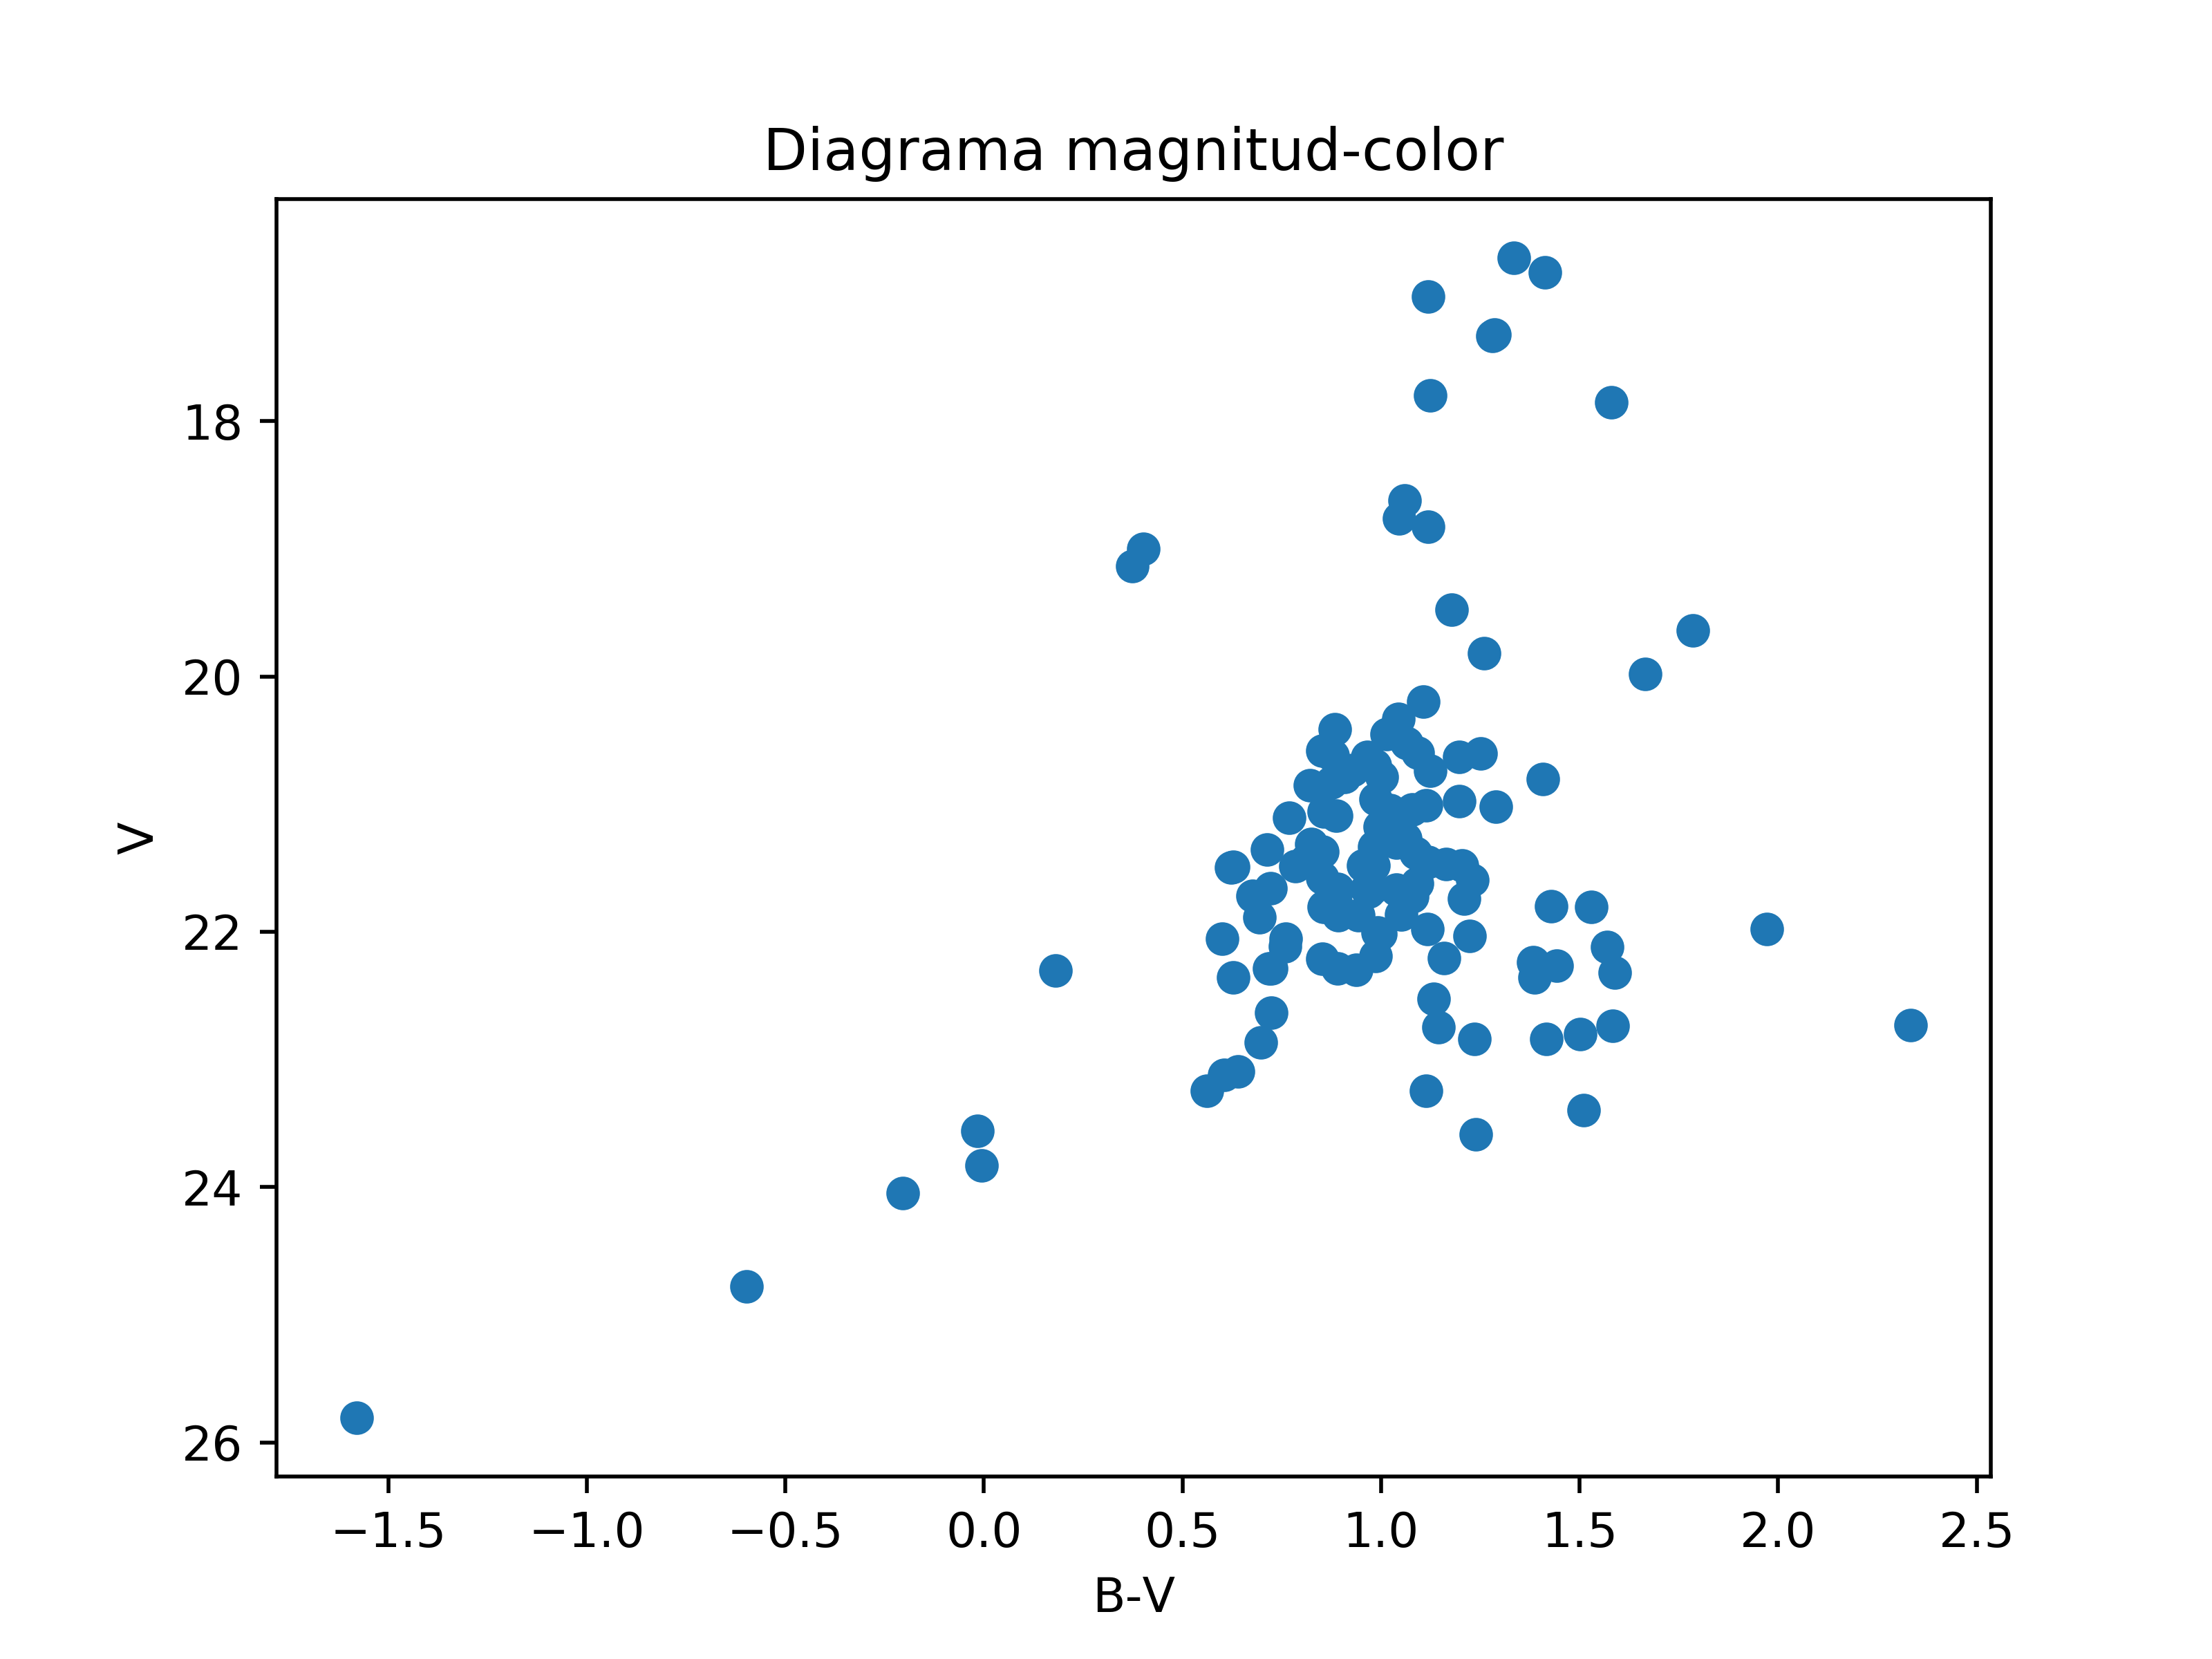
\includegraphics[width= 4.20in]{VvsBV.png}
	\caption{Diagrama magnitud-color del cúmulo M92.}
  \label{diag}
\end{figure}

\section{Fecha Juliana}
La fecha Juliana es el número de días transcurridos desde el primero de enero del año 4713 antes de Nuestra era. La fecha Juliana fue inventada en 1582 por José Scaliger con el fin de poder datar los eventos astronómicos sin tener que contar años bisiestos para el cálculo del número de días entre dos fechas. Así mismo en 1582 el calendario Gregoriano reemplaza al calendario Juliano (de uso regular en Europa desde el año 42 antes de Nuestra Era), con el nuevo calendario cambian las reglas para determinar si un año es bisiesto, por lo que se complica el cálculo de días entre dos fechas. El nuevo calendario, junto a la comodidad de un sistema continuo, llevó al establecimiento de la Fecha Juliana, dado que la fecha Juliana se usa principalmente en astronomía para la datación de eventos. Octubre 29 de 2018 es el día Juliano 2458359 .

%\bibliography{bibte}
\bibliographystyle{plain}


\end{document}




\begin{figure}[H]
  \centering
   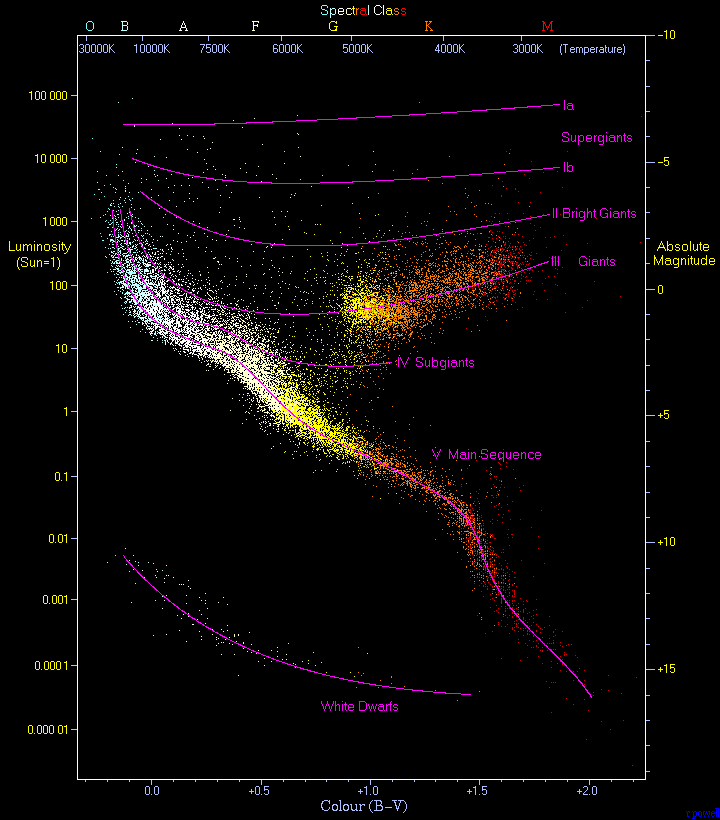
\includegraphics[width= 3.60in]{HRdiag.png}
  %\caption{Diagrama HR de 22000 estrellas del catálogo HIPPARCOS.\cite{hrdiag}  }
  \label{diag}
\end{figure}



\begin{table}[htb]
    \centering
    \label{tabla}
	\begin{tabular}{|c|c|c|c|c| }
	\hline
	Cúmulo & $E(B-V)$ & $m-M$ & Distancia [$pcs$] & Edad del cúmulo [millones de años]  \\ \hline
	NCG 752 & -0.03 & 8.02 & 401.79 & 1259  \\ \hline
	Mel 20 & +0.09 & 6.35 & 186.2 & 63  \\ \hline
	M45 & +0.04 & 5.50 & 125.89 & 126  \\ \hline
	Hyades & 0.00 & 2.84 & 36.98 & 891  \\ \hline
	M44 & +0.04 & 6.21 & 174.58 & 794  \\ \hline
	M67 & -0.03 & 9.32 & 731.14 & 5623  \\ \hline
	IC 4665 & 0.18 & 7.86 & 373.25 & 224  \\ \hline
	M39 & +0.01 & 6.87 & 238.78 & 447  \\ \hline
	\end{tabular}
\end{table}

\begin{table}[htb]
	\begin{tabular}{|c|cccccccccccccccc| }
	\hline
	Tareas $\backslash$ Semanas & 1 & 2 & 3 & 4 & 5 & 6 & 7 & 8 & 9 & 10 & 11 & 12 & 13 & 14 & 15 & 16  \\
	\hline
	1 & X & X & X  &   &   &   &   &  &  &   &   &   &   &   &   &   \\
	2 &   &  & X & X & X &  &  &   &   &  &  &  &   &  &  &   \\
	3 &   &   &   &  & X  & X  & X  & X &   &   &   &  &   &   &  &   \\
	4 &  &  &  &  &  &  &  & X & X & X & X &   &   &   &   &   \\
    5 &  &  &  &  &  &  & X & X &  &  &  &   &   &   &   &   \\
	6 &   &   &   &   &  &   &  X & X  &  &   &  X & X &  X & X  & X &   \\
	\hline
	\end{tabular}
\end{table}
\vspace{1mm}
%CCDRED se encarga de la corrección en sí, sus parámetros son: el tipo de dato de los pixeles (real, short, etc), el nombre del backup (en caso de querer un backup), el archivo de traducción del instrumento (que para una CCD estandar ya viene incluido en IRAF